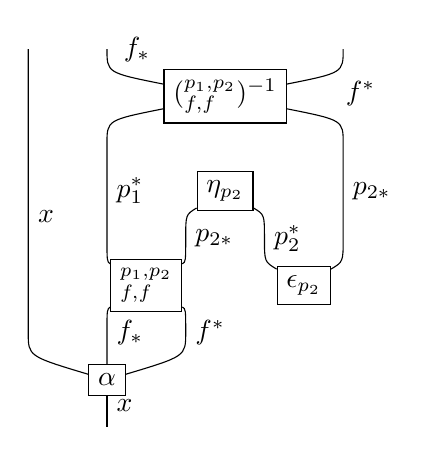
\begin{tikzpicture}[baseline=(current bounding box.center),y=0.6cm]
\path coordinate[] (tikzsd_internal_pos_0_0) at (0.0,0.0);
\path coordinate[] (tikzsd_internal_pos_0_1) at (1.0,0.0);
\path coordinate[] (tikzsd_internal_pos_0_2) at (4.0,0.0);
\path coordinate[] (tikzsd_internal_pos_1_0) at (0.0,-2.0);
\path coordinate[] (tikzsd_internal_pos_1_1) at (1.0,-2.0);
\path coordinate[] (tikzsd_internal_pos_1_2) at (4.0,-2.0);
\path coordinate[] (tikzsd_internal_pos_2_0) at (0.0,-4.0);
\path coordinate[] (tikzsd_internal_pos_2_1) at (1.0,-4.0);
\path coordinate[] (tikzsd_internal_pos_2_2) at (2.0,-4.0);
\path coordinate[] (tikzsd_internal_pos_2_3) at (3.0,-4.0);
\path coordinate[] (tikzsd_internal_pos_2_4) at (4.0,-4.0);
\path coordinate[] (tikzsd_internal_pos_3_0) at (0.0,-6.0);
\path coordinate[] (tikzsd_internal_pos_3_1) at (1.0,-6.0);
\path coordinate[] (tikzsd_internal_pos_3_2) at (2.0,-6.0);
\path coordinate[] (tikzsd_internal_pos_4_0) at (1.0,-8.0);

\path node[,draw,] (tikzsd_internal_nt_node_0_0) at (2.5,-1.0) {$(\PP_{f,f}^{p_1,p_2})^{-1}$};
\path node[,draw,] (tikzsd_internal_nt_node_1_0) at (2.5,-3.0) {$\eta_{p_2}$};
\path node[,draw,] (tikzsd_internal_nt_node_2_0) at (1.5,-5.0) {$\PP_{f,f}^{p_1,p_2}$};
\path node[,draw,] (tikzsd_internal_nt_node_2_1) at (3.5,-5.0) {$\epsilon_{p_2}$};
\path node[,draw,] (tikzsd_internal_nt_node_3_0) at (1.0,-7.0) {$\alpha$};

\path [draw] (tikzsd_internal_pos_0_0) ..controls(0.0,-0.5)and(0.0,-1.5)..(tikzsd_internal_pos_1_0) ..controls(0.0,-2.5)and(0.0,-3.5)..(tikzsd_internal_pos_2_0) node[pos=0.75,auto,] {$x$} ..controls(0.0,-4.5)and(0.0,-5.5)..(tikzsd_internal_pos_3_0) ..controls(0.0,-6.5)..(tikzsd_internal_nt_node_3_0);
\path [draw] (tikzsd_internal_pos_0_1) ..controls(1.0,-0.5)..(tikzsd_internal_nt_node_0_0) node[pos=0.5,auto,] {$f_\ast$};
\path [draw] (tikzsd_internal_pos_0_2) ..controls(4.0,-0.5)..(tikzsd_internal_nt_node_0_0) node[pos=0.5,auto,] {$f^\ast$};
\path [draw] (tikzsd_internal_nt_node_0_0) ..controls(1.0,-1.5)..(tikzsd_internal_pos_1_1) ..controls(1.0,-2.5)and(1.0,-3.5)..(tikzsd_internal_pos_2_1) node[pos=0.5,auto,] {$p_1^\ast$} ..controls(1.0,-4.5)..(tikzsd_internal_nt_node_2_0);
\path [draw] (tikzsd_internal_nt_node_1_0) ..controls(2.0,-3.5)..(tikzsd_internal_pos_2_2) ..controls(2.0,-4.5)..(tikzsd_internal_nt_node_2_0) node[pos=0.0,auto,] {$p_{2\ast}$};
\path [draw] (tikzsd_internal_nt_node_2_0) ..controls(1.0,-5.5)..(tikzsd_internal_pos_3_1) ..controls(1.0,-6.5)..(tikzsd_internal_nt_node_3_0) node[pos=0.0,auto,] {$f_\ast$};
\path [draw] (tikzsd_internal_nt_node_2_0) ..controls(2.0,-5.5)..(tikzsd_internal_pos_3_2) ..controls(2.0,-6.5)..(tikzsd_internal_nt_node_3_0) node[pos=0.0,auto,] {$f^\ast$};
\path [draw] (tikzsd_internal_nt_node_1_0) ..controls(3.0,-3.5)..(tikzsd_internal_pos_2_3) ..controls(3.0,-4.5)..(tikzsd_internal_nt_node_2_1) node[pos=0.0,auto,] {$p_2^\ast$};
\path [draw] (tikzsd_internal_nt_node_0_0) ..controls(4.0,-1.5)..(tikzsd_internal_pos_1_2) ..controls(4.0,-2.5)and(4.0,-3.5)..(tikzsd_internal_pos_2_4) node[pos=0.5,auto,] {$p_{2\ast}$} ..controls(4.0,-4.5)..(tikzsd_internal_nt_node_2_1);
\path [draw] (tikzsd_internal_nt_node_3_0) ..controls(1.0,-7.5)..(tikzsd_internal_pos_4_0) node[pos=0.5,auto,] {$x$};
\end{tikzpicture}